\chapter{Probabilistic Numerics: Nano-machine-learning by
\href{http://www.robots.ox.ac.uk/\~mosb/}{Michael A Osborne}}

9:30--11:00

Numerics is becoming one of the important fields of Machine Learning.

\begin{mybox}
  In numerical analysis, numerical integration constitutes a broad family of
  algorithms for calculating the numerical value of a definite integral, and by
  extension, the term is also sometimes used to describe the numerical solution
  of differential equations. This article focuses on calculation of definite
  integrals. The term numerical quadrature (often abbreviated to quadrature) is
  more or less a synonym for numerical integration, especially as applied to
  one-dimensional integrals. Some authors refer to numerical integration over
  more than one dimension as cubature;[1] others take quadrature to include
  higher-dimensional integration. -- Wikipedia
\end{mybox}

The answer to a numeric problem can only be approximated, e.g.

\begin{equation}
  F = \int_{-3}^3 f(x) dx
\end{equation}

for

\begin{equation}
  f(x) = \exp(-(\sin(3x))^2 - x^2)
\end{equation}

This can be as long as 30 polinomic elements. Altough we can not use it
analytically, we can get an approximated answer with a computer.

A motivation:

\begin{enumerate}
  \item numeric \emph{error} is significant
  \item numeric methods are generic
  \item our numerics problems tax our computation
\end{enumerate}

Some important parts of the integration to have in mind:

\begin{itemize}
  \item The data: are the evaluations, or
  \item Predictand: is the integral
  \item Decisions: \dots
\end{itemize}

Bayesian quadrature is probabilistic numerics for intergration

\begin{mybox}
  Bayesian Quadrature is a statistical approach to the numerical problem of
  computing integrals and falls under the field of probabilistic numerics. It
  can provide a full handling of the uncertainty over the solution of the
  integral expressed as a Gaussian Process posterior variance. It is also known
  to provide very fast convergence rates which can be up to exponential in the
  number of quadrature points n.[5] --
  \href{https://en.wikipedia.org/wiki/Numerical_integration}{Wikipedia}
\end{mybox}

With a \emph{Gaussian process} prior for the integrand, the \emph{integral is
joint Gaussian.}


\begin{figure}[h]
\centering
\pgfplotsset{
colormap={whitered}{color(0cm)=(white); color(1cm)=(orange!75!red)}
}

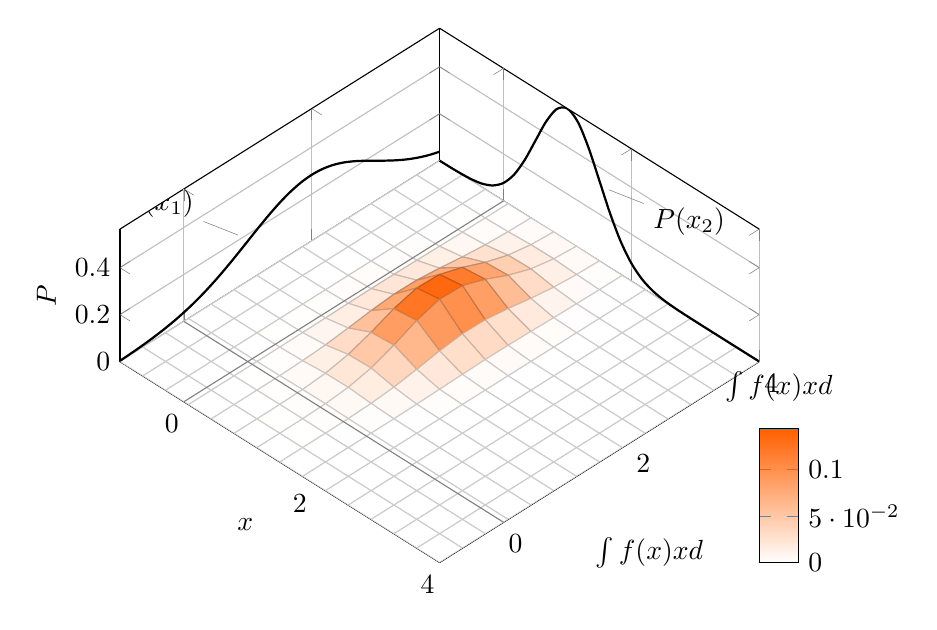
\begin{tikzpicture}[
    declare function={mu1=1;},
    declare function={mu2=2;},
    declare function={sigma1=0.5;},
    declare function={sigma2=1;},
    declare function={normal(\m,\s)=1/(2*\s*sqrt(pi))*exp(-(x-\m)^2/(2*\s^2));},
    declare function={bivar(\ma,\sa,\mb,\sb)=
        1/(2*pi*\sa*\sb) * exp(-((x-\ma)^2/\sa^2 + (y-\mb)^2/\sb^2))/2;}]
\begin{axis}[
    colormap name=whitered,
    width=.8\linewidth,
    view={45}{65},
    enlargelimits=false,
    grid=major,
    domain=-1:4,
    y domain=-1:4,
    samples=15,
    xlabel=$x$,
    ylabel=$\int f(x) xd$,
    zlabel={$P$},
    colorbar,
    colorbar style={
        at={(1,0)},
        anchor=south west,
        height=0.25*\pgfkeysvalueof{/pgfplots/parent axis height},
        title={$\int f(x) xd$}
    }
]
\addplot3 [surf] {bivar(mu1,sigma1,mu2,sigma2)};
\addplot3 [domain=-1:4,samples=31, samples y=0, thick, smooth] (x,4,{normal(mu1,sigma1)});
\addplot3 [domain=-1:4,samples=31, samples y=0, thick, smooth] (-1,x,{normal(mu2,sigma2)});

\draw [black!50] (axis cs:-1,0,0) -- (axis cs:4,0,0);
\draw [black!50] (axis cs:0,-1,0) -- (axis cs:0,4,0);

\node at (axis cs:-1,1,0.18) [pin=165:$P(x_1)$] {};
\node at (axis cs:1.5,4,0.32) [pin=-15:$P(x_2)$] {};
\end{axis}
\end{tikzpicture}
\end{figure}


Monte Carlo is also Bayesian quadrature

The motnte caro estimate is

\begin{equation}
  \int f(x) p(x) dx \backsimeq 1/N \sum_{i=1}^N f(x_i)
\end{equation}

is a maximum a-posteriori under the (imporoper) prior

\begin{equation}
  p(f) = \lim_{e \ra 0} GP(0, \theta^2 \Indicator(x = x') + c^{-1})
\end{equation}

TODO missing conclusion for last equation

Managing parameters $\theta$ requires the model \dots

\begin{equation}
  \int f(x|\theta) d\theta \text{  missing equation}
\end{equation}


In optimization it is not enought looking for the higher likelihood value, but
we are looking for the highest mass. This is picks with larga areas around.

\begin{equation}
  p(data) \backsimeq  \text{  missing}
\end{equation}

We prefer \emph{flat optima} to \emph{pick optima} preciselly because of the
mass.

In Monte Carlo estimator

\begin{equation}
  \int f(x) p(x) dx \backsimeq 1/N \sum_{i=1}^N f(x_i)
\end{equation}

ignores relevant information and assumes certain sample distribution (see Monte
  Carlo is Fundamentally unsound \cite{o1987monte})

\emph{Warped sequential active Bayesian integration (WSABI)} uses a loss that
is the uncertainty in the integrand (see Sampling for inference in
Probaiblistic models with fast bayesian quadrature, NIPS
\cite{gunter2014sampling})

\begin{mybox}
  We propose a novel sampling framework for inference in probabilistic models: an
active learning approach that converges more quickly (in wall-clock time) than
Markov chain Monte Carlo (MCMC) benchmarks. The central challenge in probabilistic
inference is numerical integration, to average over ensembles of models or
unknown (hyper-)parameters (for example to compute the marginal likelihood or
a partition function). MCMC has provided approaches to numerical integration that
deliver state-of-the-art inference, but can suffer from sample inefficiency and poor
convergence diagnostics. Bayesian quadrature techniques offer a model-based
solution to such problems, but their uptake has been hindered by prohibitive computation
costs. We introduce a warped model for probabilistic integrands (likelihoods)
that are known to be non-negative, permitting a cheap active learning
scheme to optimally select sample locations. Our algorithm is demonstrated to
offer faster convergence (in seconds) relative to simple Monte Carlo and annealed
importance sampling on both synthetic and real-world examples. -- Abstract from
\cite{gunter2014sampling}
\end{mybox}

In global optimization

\begin{itemize}
  \item Data: evaluation
  \item Predictand: minimizer
  \item Decisions: location
\end{itemize}

Bayesian optimisation is probabilistic numerics for global optimization

The loss for optimisation could be

\begin{enumerate}
  \item the lowwest evaluation (value): Some times it is really important to
    choose the best option, but not care about the uncertainty
  \item the uncertainty in the minimiser (location-information): e.g. if you
    create the model in synthetic data, it is important to evaluate the
    uncertainty on the new real data
  \item the uncertainty in the minimum (value-information):
\end{enumerate}


\begin{itemize}
    \item
    \begin{equation}
      \lambda_{VL} = y_N
    \end{equation}
    \item
    \begin{equation}
      \lambda_{LIL} = \mathbb{\mathop{M}} (x_* | x_N, y_N, D_N)
    \end{equation}
\end{itemize}

Solving the intrinsic ``myopia'' of bayesian optimization methods (see GLASSES:
relieving the myopia of bayesian optimization \cite{gonzalez2016glasses})


\section{Upper confidence bound}

is the myopic acquisition function


\begin{equation}
  \text{missing equation}
\end{equation}

given a surrogate with mean $m(x_n)$ and variance $V(x_n)$


\section{Information-theoretic methods}

give alternative myopic implementations of va-ue.-information and
location-information losses:

% \begin{align}
%   \alpha_{LiL} = \Expected_{y_n} \mathbb{\mathop{H}}(x_*|y_n, x_n, D_n)
% \end{align}

these methods tend to be more exploratory

\section{Technology at work: The future of automation Tue. 9:30--11:00}


What are humans still good for?
\bibliographystyle{apalike}
\bibliography{references}
